% Created by tikzDevice version 0.6.4 on 2013-12-02 10:08:06
% !TEX encoding = UTF-8 Unicode
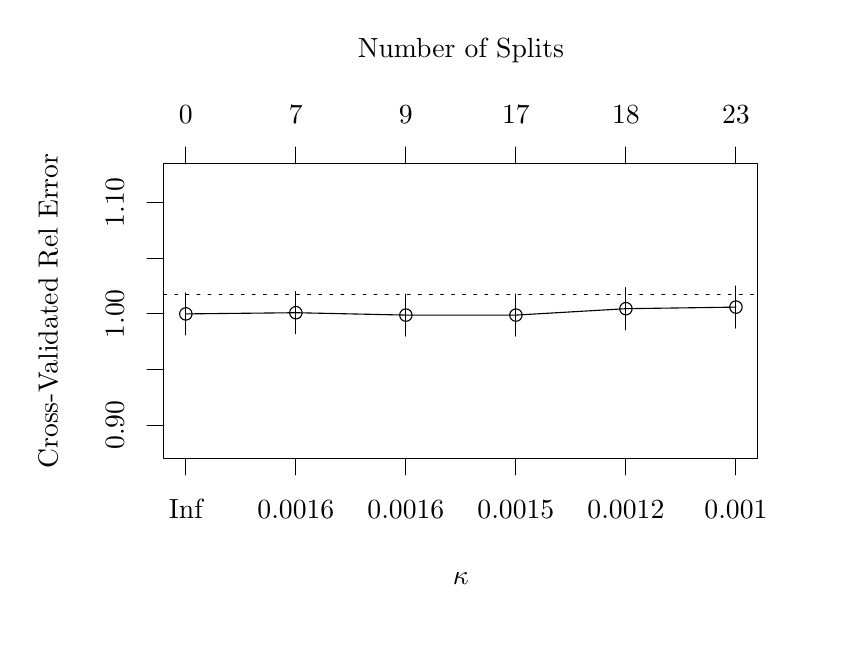
\begin{tikzpicture}[x=1pt,y=1pt]
\definecolor[named]{fillColor}{rgb}{1.00,1.00,1.00}
\path[use as bounding box,fill=fillColor,fill opacity=0.00] (0,0) rectangle (289.08,216.81);
\begin{scope}
\path[clip] ( 49.20, 61.20) rectangle (263.88,167.61);
\definecolor[named]{drawColor}{rgb}{0.00,0.00,0.00}

\path[draw=drawColor,line width= 0.4pt,line join=round,line cap=round] ( 57.15,113.38) --
	( 96.91,113.81) --
	(136.66,112.95) --
	(176.42,112.95) --
	(216.17,115.26) --
	(255.93,115.83);

\path[draw=drawColor,line width= 0.4pt,line join=round,line cap=round] ( 57.15,113.38) circle (  2.25);

\path[draw=drawColor,line width= 0.4pt,line join=round,line cap=round] ( 96.91,113.81) circle (  2.25);

\path[draw=drawColor,line width= 0.4pt,line join=round,line cap=round] (136.66,112.95) circle (  2.25);

\path[draw=drawColor,line width= 0.4pt,line join=round,line cap=round] (176.42,112.95) circle (  2.25);

\path[draw=drawColor,line width= 0.4pt,line join=round,line cap=round] (216.17,115.26) circle (  2.25);

\path[draw=drawColor,line width= 0.4pt,line join=round,line cap=round] (255.93,115.83) circle (  2.25);
\end{scope}
\begin{scope}
\path[clip] (  0.00,  0.00) rectangle (289.08,216.81);
\definecolor[named]{drawColor}{rgb}{0.00,0.00,0.00}

\node[text=drawColor,anchor=base,inner sep=0pt, outer sep=0pt, scale=  1.00] at (156.54, 15.60) {$\kappa$};

\node[text=drawColor,rotate= 90.00,anchor=base,inner sep=0pt, outer sep=0pt, scale=  1.00] at ( 10.80,114.40) {Cross-Validated Rel Error};
\end{scope}
\begin{scope}
\path[clip] (  0.00,  0.00) rectangle (289.08,216.81);
\definecolor[named]{drawColor}{rgb}{0.00,0.00,0.00}

\path[draw=drawColor,line width= 0.4pt,line join=round,line cap=round] ( 49.20, 61.20) --
	(263.88, 61.20) --
	(263.88,167.61) --
	( 49.20,167.61) --
	( 49.20, 61.20);

\path[draw=drawColor,line width= 0.4pt,line join=round,line cap=round] ( 49.20, 73.16) -- ( 49.20,153.60);

\path[draw=drawColor,line width= 0.4pt,line join=round,line cap=round] ( 49.20, 73.16) -- ( 43.20, 73.16);

\path[draw=drawColor,line width= 0.4pt,line join=round,line cap=round] ( 49.20, 93.27) -- ( 43.20, 93.27);

\path[draw=drawColor,line width= 0.4pt,line join=round,line cap=round] ( 49.20,113.38) -- ( 43.20,113.38);

\path[draw=drawColor,line width= 0.4pt,line join=round,line cap=round] ( 49.20,133.49) -- ( 43.20,133.49);

\path[draw=drawColor,line width= 0.4pt,line join=round,line cap=round] ( 49.20,153.60) -- ( 43.20,153.60);

\node[text=drawColor,rotate= 90.00,anchor=base,inner sep=0pt, outer sep=0pt, scale=  1.00] at ( 34.80, 73.16) {0.90};

\node[text=drawColor,rotate= 90.00,anchor=base,inner sep=0pt, outer sep=0pt, scale=  1.00] at ( 34.80,113.38) {1.00};

\node[text=drawColor,rotate= 90.00,anchor=base,inner sep=0pt, outer sep=0pt, scale=  1.00] at ( 34.80,153.60) {1.10};
\end{scope}
\begin{scope}
\path[clip] ( 49.20, 61.20) rectangle (263.88,167.61);
\definecolor[named]{drawColor}{rgb}{0.00,0.00,0.00}

\path[draw=drawColor,line width= 0.4pt,line join=round,line cap=round] ( 57.15,105.79) -- ( 57.15,120.97);

\path[draw=drawColor,line width= 0.4pt,line join=round,line cap=round] ( 96.91,106.22) -- ( 96.91,121.41);

\path[draw=drawColor,line width= 0.4pt,line join=round,line cap=round] (136.66,105.36) -- (136.66,120.53);

\path[draw=drawColor,line width= 0.4pt,line join=round,line cap=round] (176.42,105.36) -- (176.42,120.53);

\path[draw=drawColor,line width= 0.4pt,line join=round,line cap=round] (216.17,107.65) -- (216.17,122.87);

\path[draw=drawColor,line width= 0.4pt,line join=round,line cap=round] (255.93,108.22) -- (255.93,123.45);
\end{scope}
\begin{scope}
\path[clip] (  0.00,  0.00) rectangle (289.08,216.81);
\definecolor[named]{drawColor}{rgb}{0.00,0.00,0.00}

\path[draw=drawColor,line width= 0.4pt,line join=round,line cap=round] ( 57.15, 61.20) -- (255.93, 61.20);

\path[draw=drawColor,line width= 0.4pt,line join=round,line cap=round] ( 57.15, 61.20) -- ( 57.15, 55.20);

\path[draw=drawColor,line width= 0.4pt,line join=round,line cap=round] ( 96.91, 61.20) -- ( 96.91, 55.20);

\path[draw=drawColor,line width= 0.4pt,line join=round,line cap=round] (136.66, 61.20) -- (136.66, 55.20);

\path[draw=drawColor,line width= 0.4pt,line join=round,line cap=round] (176.42, 61.20) -- (176.42, 55.20);

\path[draw=drawColor,line width= 0.4pt,line join=round,line cap=round] (216.17, 61.20) -- (216.17, 55.20);

\path[draw=drawColor,line width= 0.4pt,line join=round,line cap=round] (255.93, 61.20) -- (255.93, 55.20);

\node[text=drawColor,anchor=base,inner sep=0pt, outer sep=0pt, scale=  1.00] at ( 57.15, 39.60) {Inf};

\node[text=drawColor,anchor=base,inner sep=0pt, outer sep=0pt, scale=  1.00] at ( 96.91, 39.60) {0.0016};

\node[text=drawColor,anchor=base,inner sep=0pt, outer sep=0pt, scale=  1.00] at (136.66, 39.60) {0.0016};

\node[text=drawColor,anchor=base,inner sep=0pt, outer sep=0pt, scale=  1.00] at (176.42, 39.60) {0.0015};

\node[text=drawColor,anchor=base,inner sep=0pt, outer sep=0pt, scale=  1.00] at (216.17, 39.60) {0.0012};

\node[text=drawColor,anchor=base,inner sep=0pt, outer sep=0pt, scale=  1.00] at (255.93, 39.60) {0.001};

\path[draw=drawColor,line width= 0.4pt,line join=round,line cap=round] ( 57.15,167.61) -- (255.93,167.61);

\path[draw=drawColor,line width= 0.4pt,line join=round,line cap=round] ( 57.15,167.61) -- ( 57.15,173.61);

\path[draw=drawColor,line width= 0.4pt,line join=round,line cap=round] ( 96.91,167.61) -- ( 96.91,173.61);

\path[draw=drawColor,line width= 0.4pt,line join=round,line cap=round] (136.66,167.61) -- (136.66,173.61);

\path[draw=drawColor,line width= 0.4pt,line join=round,line cap=round] (176.42,167.61) -- (176.42,173.61);

\path[draw=drawColor,line width= 0.4pt,line join=round,line cap=round] (216.17,167.61) -- (216.17,173.61);

\path[draw=drawColor,line width= 0.4pt,line join=round,line cap=round] (255.93,167.61) -- (255.93,173.61);

\node[text=drawColor,anchor=base,inner sep=0pt, outer sep=0pt, scale=  1.00] at ( 57.15,182.01) {0};

\node[text=drawColor,anchor=base,inner sep=0pt, outer sep=0pt, scale=  1.00] at ( 96.91,182.01) {7};

\node[text=drawColor,anchor=base,inner sep=0pt, outer sep=0pt, scale=  1.00] at (136.66,182.01) {9};

\node[text=drawColor,anchor=base,inner sep=0pt, outer sep=0pt, scale=  1.00] at (176.42,182.01) {17};

\node[text=drawColor,anchor=base,inner sep=0pt, outer sep=0pt, scale=  1.00] at (216.17,182.01) {18};

\node[text=drawColor,anchor=base,inner sep=0pt, outer sep=0pt, scale=  1.00] at (255.93,182.01) {23};

\node[text=drawColor,anchor=base,inner sep=0pt, outer sep=0pt, scale=  1.00] at (156.54,206.01) {Number of Splits};
\end{scope}
\begin{scope}
\path[clip] ( 49.20, 61.20) rectangle (263.88,167.61);
\definecolor[named]{drawColor}{rgb}{0.00,0.00,0.00}

\path[draw=drawColor,line width= 0.4pt,dash pattern=on 1pt off 3pt ,line join=round,line cap=round] ( 49.20,120.53) -- (263.88,120.53);
\end{scope}
\end{tikzpicture}
